\documentclass{beamer}

\usepackage{amsmath}
\usepackage{cancel}
\usepackage{mathtools}
\usepackage{multirow}
\usepackage{tikz, pgfplots}
\pgfplotsset{compat=1.18}

\title{Applying the Klein-Gordon Theory to Gravitation}

\subtitle{Modelling Newtonian gravitation as a classical scalar field theory obeying Klein-Gordon structure}

\author{Siddhartha Bhattacharjee}

\institute
{
1B Mathematical Physics \\
University of Waterloo
}

\date{SASMS, Feb 10, 2023}

\begin{document}

\frame{\titlepage}

\begin{frame}
\frametitle{Table of Contents}
\tableofcontents
\end{frame}

\section{Towards Classical Field Theory}

\begin{frame}
\begin{center}
\huge \textcolor{blue!50!gray}{Towards Classical Field Theory}
\end{center}
\end{frame}

\begin{frame}
\frametitle{The Inverse Square Law}

\begin{itemize}
\item Gravitational force:
\end{itemize}

$$F_m = - G \frac{M m}{r^2}$$

\begin{itemize}
\item Electrostatic force:
\end{itemize}

$$F_e = \frac{1}{4 \pi \epsilon_0} \frac{Q_e q_e}{r^2}$$

\begin{itemize}
\item Magnetic force:
\end{itemize}

$$F_b = \frac{\mu_0}{4 \pi} \frac{Q_b q_b}{r^2}$$
\end{frame}

\subsection{Formal Analogies Between the Gravitational and Electrostatic Forces}

\begin{frame}
\frametitle{Formal Analogies Between the Gravitational and Electrostatic Forces}

\begin{center}
\begin{tabular}{ |c|c|c|c| } 
\hline
& Gravitation & Static electricity \\
\hline
Newton's second law & $a^i = \underset{- \vec{\nabla} V}{\underbrace{- \partial^i V}}$ & $E^i = \underset{- \vec{\nabla} \phi}{\underbrace{- \partial^i \phi}}$ \\
\hline
Gauss' law & $\underset{\vec{\nabla} \cdot \vec{a}}{\underbrace{\sum \limits_{i=1}^3 \nabla_i a^i}} = - 4 \pi G \rho_m$ & $\underset{\vec{\nabla} \cdot \vec{a}}{\underbrace{\sum \limits_{i=1}^3 \nabla_i E^i}} = \frac{1}{\epsilon_0} \rho_e$ \\
\hline
Poisson's equation & $\underset{\nabla^2 V}{\underbrace{\sum \limits_{i=1}^3 \nabla_i \partial^i V}} = 4 \pi G \rho_m$ & $\underset{\nabla^2 \phi}{\underbrace{\sum \limits_{i=1}^3 \nabla_i \partial^i \phi}} = - \frac{1}{\epsilon_0} \rho_e$ \\  
\hline
\end{tabular}
\end{center}
\end{frame}

\subsection{Classical Mechanics}

\begin{frame}
\frametitle{Lagrangian Mechanics}

\begin{center}
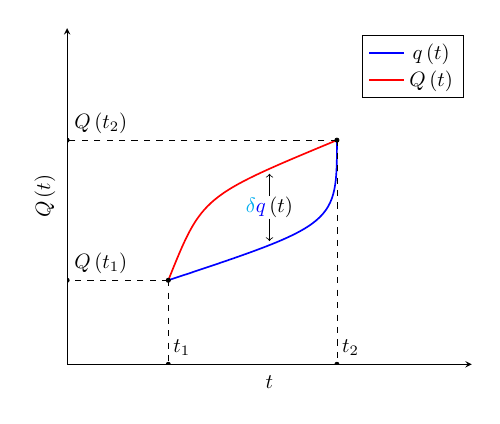
\begin{tikzpicture}[scale=0.75]
\begin{axis}[
    axis lines = left,
    xlabel = $t$,
    ylabel = $Q \left( t \right)$,
    xtick = \empty,
    ytick = \empty,
    xmin=0, xmax=3,
    ymin=0, ymax=3,
]

\draw[thick, blue] (0.75, 0.75) .. controls (2, 1.25) .. (2, 2);
\addlegendimage{thick, color=blue};
\addlegendentry{$q \left( t \right)$};

\draw[thick, red] (0.75, 0.75) .. controls (1, 1.5) .. (2, 2);
\addlegendimage{thick, color=red};
\addlegendentry{$Q \left( t \right)$};

\draw[->] (1.5, 1.5) to (1.5, 1.7);
\draw[->] (1.5, 1.3) to (1.5, 1.1);
\node[] at (1.5, 1.4) {$\textcolor{cyan}{\delta} \textcolor{blue}{q} \left( t \right)$};

\draw[dashed] (0.75, 0.75) -- (0.75, 0);
\draw[dashed] (0.75, 0.75) -- (0, 0.75);
\draw[dashed] (2, 2) -- (2, 0);
\draw[dashed] (2, 2) -- (0, 2);
\node[] at (0.85, 0.15) {$t_1$};
\node[] at (2.1, 0.15) {$t_2$};
\node[] at (0.25, 0.9) {$Q \left( t_1 \right)$};
\node[] at (0.25, 2.15) {$Q \left( t_2 \right)$};

\filldraw[] (0.75, 0.75) circle (1 pt);
\filldraw (2, 2) circle (1 pt);
\filldraw (0.75, 0) circle (1 pt);
\filldraw (0, 0.75) circle (1 pt);
\filldraw (2, 0) circle (1 pt);
\filldraw (0, 2) circle (1 pt);

\end{axis}
\end{tikzpicture}
\end{center}

\begin{itemize}
\item Nature 'selects' the unique on-shell trajectory $\textcolor{blue}{q \left( t \right)}$ given the boundary conditions $\left( t_1, \textcolor{red}{Q \left( t_1 \right)} \right)$ and $\left( t_2, \textcolor{red}{Q \left( t_2 \right)} \right)$ for a system.
\end{itemize}

\begin{align*}
\underset{\text{Off-shell}}{\underbrace{\textcolor{red}{Q \left( t \right)}}} & = \underset{\text{On-shell}}{\underbrace{\textcolor{blue}{q \left( t \right)}}} + \underset{\text{Variation}}{\underbrace{\textcolor{cyan}{\delta} \textcolor{blue}{q} \left( t \right)}} \\
\textcolor{cyan}{\delta} \textcolor{blue}{q \left( t_1 \right)} & = \textcolor{cyan}{\delta} \textcolor{blue}{q \left( t_2 \right)} = 0
\end{align*}
\end{frame}

\begin{frame}
\begin{itemize}
\item Each trajectory $\textcolor{red}{Q \left( t \right)}$ between the endpoints is associated with a corresponding number called the action.

$$\boxed{S \left[ \textcolor{red}{Q \left( t \right)} \right] \left( t_1, t_2 \right) = \int_{t_1}^{t_2} dt \: L \left( \textcolor{red}{Q \left( t \right)}, \textcolor{red}{\dot{Q} \left( t \right)}, t \right)}$$

The integrand $L \left( \textcolor{red}{Q \left( t \right)}, \textcolor{red}{\dot{Q} \left( t \right)}, t \right)$ is known as the Lagrangian of the system being modelled and encodes the dynamics of the system.

\item In general, the action $S$ maps $\textcolor{red}{Q \left( t \right)}$ to a real number determined by the above integral. Therefore, it is a functional, i.e. a higher-order function which takes in infinite values of the form $\left\{ \left( t, \textcolor{red}{Q \left( t \right)} \right) : t \in \mathbb{R} \right\}$ and spits out a real.
\end{itemize}

$$
S : \begin{cases} \mathbb{R}^\mathbb{R} & \to \mathbb{R} \\ \textcolor{red}{Q \left( t \right)} & \mapsto \displaystyle{\int}_{t_1}^{t_2} dt \: L \left( \textcolor{red}{Q \left( t \right)}, \textcolor{red}{\dot{Q} \left( t \right)}, t \right) \end{cases}
$$
\end{frame}

\begin{frame}
\frametitle{Principle of Stationary Action}

\begin{block}{Lagrange's principle of stationary action}
Suppose we vary $\textcolor{blue}{q \left( t \right)}$ about its on-shell evolution as, $\textcolor{blue}{q \left( t \right)} \to \textcolor{blue}{q \left( t \right)} + \textcolor{cyan}{\delta} \textcolor{blue}{q} \left( t \right)$. Then, the variation in the action satisfies,

$$\textcolor{cyan}{\delta} S \in \mathcal{O} \left( \textcolor{cyan}{\delta} \textcolor{blue}{q}^2  \right)$$
\end{block}

\begin{corollary}[First-order approximation]
For very small $\delta q \left( t \right)$ i.e.,

\begin{align*}
\forall \: \textcolor{cyan}{\delta} \textcolor{blue}{q} \left( t \right) & = \lim_{\textcolor{cyan}{\epsilon} \to 0} \textcolor{cyan}{\epsilon} \eta \left( t \right) : \eta \left( t_1 \right) = \eta \left( t_2 \right) = 0 : \\
\textcolor{cyan}{\delta} S & \in \mathcal{O} \left( \textcolor{cyan}{\epsilon^2} \eta \left( t \right) \right) = \left\{ 0 \right\} \\
& \implies \boxed{\textcolor{cyan}{\delta} S = 0}
\end{align*}
\end{corollary}
\end{frame}

\begin{frame}
\frametitle{Euler-Lagrange Equation}

\begin{lemma}[Fundamental lemma of calculus of variations]
The former is possible if and only if the latter is,

\begin{align*}
\forall \: \textcolor{cyan}{\delta} \textcolor{blue}{q} : \int_{t_1}^{t_2} dt \: \textcolor{cyan}{\delta} \textcolor{blue}{q} \: f \left( \textcolor{blue}{q}, \textcolor{blue}{\dot{q}}, t \right) & = 0 \\
\Longleftrightarrow \forall \: t \in \left( t_1, t_2 \right) : f \left( \textcolor{blue}{q}, \textcolor{blue}{\dot{q}}, t \right) & = 0
\end{align*}
\end{lemma}

\begin{theorem}
An on-shell $\textcolor{blue}{q \left( t \right)}$ obeying the principle of stationary action for a given $L \left( \textcolor{blue}{q}, \textcolor{blue}{\dot{q}}, t \right)$ must also obey the Euler-Lagrange equation of motion:

$$\boxed{\underset{\text{Generalized force}}{\underbrace{\frac{\partial L}{\partial \textcolor{blue}{q}}}} = \underset{\text{Conjugate momentum}}{\frac{d}{dt} \underbrace{\frac{\partial L}{\partial \textcolor{blue}{\dot{q}}}}} = \frac{d \textcolor{blue}{p}}{dt}}$$
\end{theorem}
\end{frame}

\begin{frame}
\begin{block}{Proof.}
\begin{align*}
\textcolor{cyan}{\delta} S & = 0 & \left[ \text{Principle of stationary action} \right] \\
\textcolor{cyan}{\delta} \int_{t_1}^{t_2} dt \: L \left( \textcolor{blue}{q}, \textcolor{blue}{\dot{q}}, t \right) & = 0 \\
\int_{t_1}^{t_2} dt \: \textcolor{cyan}{\delta} L \left( \textcolor{blue}{q}, \textcolor{blue}{\dot{q}}, t \right) & = 0 & \left[ \text{Additivity of variations} \right] \\
\int_{t_1}^{t_2} dt \left[  \textcolor{cyan}{\delta} \textcolor{blue}{q} \frac{\partial L}{\partial \textcolor{blue}{q}} + \textcolor{cyan}{\delta} \textcolor{blue}{\dot{q}} \frac{\partial L}{\partial \textcolor{blue}{\dot{q}}} + \cancel{\textcolor{cyan}{\delta} t} \frac{\partial L}{\partial t} \right] & = 0 & \left[ \text{Chain rule for variations} \right] \\
\int_{t_1}^{t_2} dt \left[  \textcolor{cyan}{\delta} \textcolor{blue}{q} \frac{\partial L}{\partial \textcolor{blue}{q}} + \dot{\left( \textcolor{cyan}{\delta} \textcolor{blue}{{q}}\right)} \frac{\partial L}{\partial \textcolor{blue}{\dot{q}}} \right] & = 0 & \left[ \text{Commutativity of derivatives} \right] \\
\int_{t_1}^{t_2} dt \: \textcolor{cyan}{\delta} \textcolor{blue}{q} \frac{\partial L}{\partial \textcolor{blue}{q}} + \int_{t_1}^{t_2} dt \: \dot{\left( \textcolor{cyan}{\delta} \textcolor{blue}{{q}}\right)} \frac{\partial L}{\partial \textcolor{blue}{\dot{q}}} & = 0
\end{align*}
\end{block}
\end{frame}

\begin{frame}
\begin{block}{Proof.}
\begin{align*}
\int_{t_1}^{t_2} dt \: \textcolor{cyan}{\delta} \textcolor{blue}{q} \frac{\partial L}{\partial \textcolor{blue}{q}} + \frac{\partial L}{\partial \textcolor{blue}{\dot{q}}} \int_{t_1}^{t_2} dt \: \dot{\left( \textcolor{cyan}{\delta} \textcolor{blue}{{q}}\right)} - \int_{t_1}^{t_2} dt \left[ \int dt \: \dot{\left( \textcolor{cyan}{\delta} \textcolor{blue}{{q}}\right)} \right] \frac{d}{dt} \frac{\partial L}{\partial \textcolor{blue}{\dot{q}}} & = 0 \\
\left[ \text{Integration by parts} \right] \\
\int_{t_1}^{t_2} dt \: \textcolor{cyan}{\delta} \textcolor{blue}{q} \frac{\partial L}{\partial \textcolor{blue}{q}} + \frac{\partial L}{\partial \textcolor{blue}{\dot{q}}} \cancel{\left[ \textcolor{cyan}{\delta} \textcolor{blue}{{q}}\right]}_{t_1}^{t_2} - \int_{t_1}^{t_2} dt \: \textcolor{cyan}{\delta} \textcolor{blue}{q} \frac{d}{dt} \frac{\partial L}{\partial \textcolor{blue}{\dot{q}}} & = 0 \\
\left[ \textcolor{cyan}{\delta} \textcolor{blue}{q} \left( t_1 \right) = \textcolor{cyan}{\delta} \textcolor{blue}{q} \left( t_2 \right) \right] \\
\forall \: \textcolor{cyan}{\delta} \textcolor{blue}{q} : \int_{t_1}^{t_2} dt \textcolor{cyan}{\delta} \textcolor{blue}{q} \left( \frac{\partial L}{\partial \textcolor{blue}{q}} - \frac{d}{dt} \frac{\partial L}{\partial \textcolor{blue}{\dot{q}}} \right) & = 0 \\
\Longleftrightarrow \frac{\partial L}{\partial \textcolor{blue}{q}} - \frac{d}{dt} \frac{\partial L}{\partial \textcolor{blue}{\dot{q}}} & = 0 \\
\Longleftrightarrow \frac{\partial L}{\partial \textcolor{blue}{q}} - \frac{d \textcolor{blue}{p}}{dt} & = 0 & \square \\
\left[ \text{Fundamental lemma of the calculus of variations} \right]
\end{align*}
\end{block}
\end{frame}

\begin{frame}
\frametitle{Noether's Theorem}

\begin{theorem}[Noether's first theorem]
If the action $S \left[ \textcolor{blue}{q \left( t \right)} \right]$ remains invariant under perturbations of the following form,

$$\textcolor{blue}{q} \to \textcolor{blue}{q} + \textcolor{cyan}{\delta} \textcolor{blue}{q}$$

then the following quantity is conserved,

\begin{align*}
j & = \textcolor{blue}{p} \: \textcolor{cyan}{\delta} \textcolor{blue}{q} \\
\frac{dj}{dt} & = 0
\end{align*}
\end{theorem}
\end{frame}

\begin{frame}
\begin{block}{Proof.}
\begin{align*}
\textcolor{cyan}{\delta} L & = \frac{\partial L}{\partial \textcolor{blue}{q}} \textcolor{cyan}{\delta} \textcolor{blue}{q} + \frac{\partial L}{\partial \textcolor{blue}{\dot{q}}} \textcolor{cyan}{\delta} \textcolor{blue}{\dot{q}} \\
& = \dot{p} \textcolor{cyan}{\delta} \textcolor{blue}{q} + p \textcolor{cyan}{\delta} \textcolor{blue}{\dot{q}} & \left[ \text{Euler-Lagrange equation} \right] \\
& = \frac{d}{dt} \left( p \textcolor{cyan}{\delta} \textcolor{blue}{q} \right) \\
\text{But} \: \textcolor{cyan}{\delta} L & = 0 \\
\implies \frac{d}{dt} \left( p \textcolor{cyan}{\delta} \textcolor{blue}{q} \right) & = 0 & \square
\end{align*}
\end{block}

\begin{example}
If $S \left[ \textcolor{blue}{q \left( t \right)} \right]$ is symmetric (i.e. conserved) under a small time-independent translation $\textcolor{blue}{q} \to \textcolor{blue}{q} + \textcolor{cyan}{\epsilon}$, we obtain the invariant $j = \textcolor{blue}{p} \textcolor{cyan}{\epsilon}$. Since $\frac{dj}{dt} = 0, \frac{d \textcolor{cyan}{\epsilon}}{dt} = 0$, we get $\frac{d \textcolor{blue}{p}}{dt} = 0$.
\end{example}
\end{frame}

\begin{frame}
\frametitle{Classical Mechanics}

\begin{itemize}
\item The Lagrangian for classical mechanics is of the form,
\end{itemize}

\begin{align*}
L \left( q, \dot{q}, t \right) & = T \left( \dot{q} \right) - V \left( q \right) \\
& = \frac{1}{2} m \mathit{g} \dot{q}^2 - V \left( q \right) \\
& = \frac{1}{2} mv^2 - V \left( q \right)
\end{align*}

\begin{itemize}
\item The equation of motion obtained by applying the Euler-Lagrange equation to the above Lagrangian is,

$$\frac{d}{dt} \left( m v \right) + \frac{\partial V}{\partial q} = 0$$

This is Newton's second law. If the entire system concerned is symmetric under small translations on $q$, we have $\frac{\partial V}{\partial q} = 0$ implying $\frac{d}{dt} \left( m v \right) = 0$. This is Newton's third law.
\end{itemize}
\end{frame}

\subsection{Classical Field Theory}

\begin{frame}
\frametitle{Classical Field Theory}

\begin{itemize}
\item A classical field is a tensor field on spacetime (which is a pseudo-Riemannian manifold obeying dynamical field equations such as the Einstein field equations).

Therefore, a classical field is some rank $\left( p, q \right)$ tensor $\phi^{\mu_1 \dots \mu_p}_{\phantom{\mu_1 \dots \mu_p} \nu_1 \dots \nu_q} \left( x^\alpha \right)$ at each point $x^\alpha$ in space and time with $\alpha \in \left( 0, 1, 2, 3 \right)$.

\item A classical field obeys the following principles:

\begin{enumerate}
\item Principle of stationary action

\item Local Lorentz invariance

\item Locality

\item Gauge invariance
\end{enumerate}

\item The simplest classical field theory is that of rank $\left( 0, 0 \right)$ tensor fields i.e. scalar fields $\phi \left( x^\alpha \right)$, in a flat spacetime $\mathcal{M}$. We will study such fields in the following slides.
\end{itemize}
\end{frame}

\begin{frame}
\frametitle{Principle of Stationary Action for Classical Fields}

\begin{center}
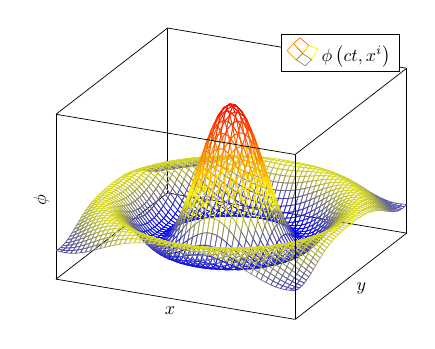
\begin{tikzpicture}[scale=0.65]
\begin{axis}[
xlabel = $x$,
ylabel = $y$,
zlabel = $\phi$,
xtick = \empty,
ytick = \empty,
ztick = \empty,
3d box = complete*,
]
 
\addplot3[
mesh,
samples=50,
domain=-8:8,
]
{sin(deg(sqrt(x^2+y^2)))/sqrt(x^2+y^2)};
\addlegendentry{$\phi \left( ct, x^i \right)$} 

\end{axis}
\end{tikzpicture}
\end{center}

\begin{itemize}
\item To construct the action for a particle, we integrated its Lagrangian between endpoints in time. A field such as $\phi \left( x^\alpha \right)$, however, lives in space and time. Therefore, its action is a \emph{volume} integral of a Lagrangian \emph{density} $\mathcal{L}$, in a 4-dimensional region of spacetime $\Omega \subset \mathcal{M}$,

$$\boxed{S \left[ \phi \left( x^\alpha \right) \right] = \int_\Omega d^4 x \: \mathcal{L} \left( \phi \left( x^\alpha \right), \partial_\mu \phi \left( x^\alpha \right), x^\nu \right)}$$
\end{itemize}
\end{frame}

\begin{frame}
\begin{itemize}
\item The Lagrangian density is so-called as it looks like a Lagrangian (integrable over some time interval $\Omega^{\left( 1 \right)}$) when integrated over a region of space $\Omega^{\left( 3 \right)}$:

\begin{align*}
L \left( \phi \left( x^\alpha \right), \partial_\mu \phi \left( x^\alpha \right), x^\nu \right) & = \int_{\Omega^{\left( 3 \right)}} d^3 x \: \mathcal{L} \left( \phi \left( x^\alpha \right), \partial_\mu \phi \left( x^\alpha \right), x^\nu \right) \\
S \left[ \phi \left( x^\alpha \right) \right] & = \int_\Omega d^4 x \: \mathcal{L} \left( \phi \left( x^\alpha \right), \partial_\mu \phi \left( x^\alpha \right), x^\nu \right) \\
& = \int_{\Omega^{\left( 1 \right)}} c dt \: L \left( \phi \left( x^\alpha \right), \partial_\mu \phi \left( x^\alpha \right), x^\nu \right)
\end{align*}

\item The principle of stationary action for fields states that for small variations $\delta \phi$ of a field $\phi$ in its on-shell configuration, the action remains stationary,

$$\boxed{\delta S = 0}$$
\end{itemize}
\end{frame}

\begin{frame}
\frametitle{Euler-Lagrange Equation for Classical Fields}

\begin{lemma}[Fundamental lemma of multivariable calculus of variations]

\begin{align*}
\forall \: \delta \phi : \int_{\Omega} d^4 x \delta \phi \: f \left( \phi, \partial_\mu \phi, x^\nu \right) & = 0 \\
\Longleftrightarrow \forall \: x^\alpha \in \Omega \backslash \partial \Omega : f \left( \phi, \partial_\mu \phi, x^\nu \right) & = 0
\end{align*}
\end{lemma}

\begin{block}{Einstein summation convention}

Dummy indices, i.e. pairs of upper and lower tensor indices, are implicitly summed over.
\end{block}

\begin{example}
$$A_\mu B^\mu = \sum_{\mu=0}^3 A_\mu B^\mu$$
\end{example}
\end{frame}

\begin{frame}
\begin{Theorem}
A field $\phi$ obeys the principle of stationary action if and only if it also satisfies,

$$\boxed{\frac{\partial \mathcal{L}}{\partial \phi} = \underset{\text{Conjugate momentum tensor}}{\nabla_\mu \underbrace{\frac{\partial \mathcal{L}}{\partial \left( \partial_\mu \phi \right)}}} = \nabla_\mu \pi^\mu}$$
\end{Theorem}

\begin{block}{Proof.}
\begin{align*}
\delta S & = 0 & \left[ \text{Principle of stationary action} \right] \\
\delta \int_\Omega d^4 x \: \mathcal{L} & = 0 \\
\int_\Omega d^4 x \: \delta \mathcal{L} & = 0 & \left[ \text{Additivity of variations} \right]
\end{align*}
\end{block}
\end{frame}

\begin{frame}
\begin{align*}
\int_\Omega d^4 x \left[ \delta \phi \frac{\partial \mathcal{L}}{\partial \phi} + \delta \left( \partial_\mu \phi \right) \underset{\pi^\mu}{\underbrace{\frac{\partial \mathcal{L}}{\partial \left( \partial_\mu \phi \right)}}} + \cancel{\delta x^\mu} \partial_\mu \mathcal{L} \right] & = 0 \\
\left[ \text{Multivariable chain rule for variations} \right] \\
\int_\Omega d^4 x \left[ \delta \phi \frac{\partial \mathcal{L}}{\partial \phi} + \left( \partial_\mu \delta \phi \right) \pi^\mu \right] & = 0 \\
\left[ \text{Commutativity of variations and covariant derivatives} \right] \\
\int_\Omega d^4 x \: \delta \phi \frac{\partial \mathcal{L}}{\partial \phi} + \pi^\mu \underset{\text{Constant surface term}}{\underbrace{\int_\Omega d^4 x \: \partial_\mu \delta \phi}} - \int_\Omega d^4 x \left[ \int d^4 x \: \partial_\mu \delta \phi \right] \nabla_\mu \pi^\mu & = 0 \\
\left[ \text{Volume integration by parts} \right] \\
\end{align*}
\end{frame}

\begin{frame}
Using Stokes' theorem, the constant surface term can be set to $0$. We then find,

\begin{align*}
\int_\Omega d^4 x \: \delta \phi \frac{\partial \mathcal{L}}{\partial \phi} - \int_\Omega d^4 x \: \delta \phi \: \nabla_\mu \pi^\mu & = 0 \\
\int_\Omega d^4 x \: \delta \phi \left( \frac{\partial \mathcal{L}}{\partial \phi} - \nabla_\mu \pi^\mu \right) & = 0 \\
\frac{\partial \mathcal{L}}{\partial \phi} - \nabla_\mu \pi^\mu & = 0 \\
\Longleftrightarrow \frac{\partial \mathcal{L}}{\partial \phi} - \nabla_\mu \frac{\partial \mathcal{L}}{\partial \left( \partial_\mu \phi \right)} & = 0 & \square \\
\left[ \text{Fundamental lemma of multivariable calculus of variations} \right]
\end{align*}
\end{frame}

\begin{frame}
\frametitle{Noether's Theorem for Classical Fields}

\end{frame}

\end{document}